%!TEX root = ../main.tex
%%%%%%%%%%%%%%%%%%%%%%%%%%%%%%%%%%
% Links:
%
% Difficulty: Companies: 
%%%%%%%%%%%%%%%%%%%%%%%%%%%%%%%%%%


%\begin{figure} \centering
%   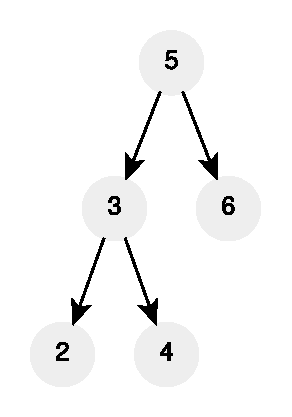
\includegraphics[width=\textwidth]{sources/next_greater_element/images/example1} \caption[Sample
%   short cpation]{Sample Caption}. \label{fig:next_greater_element:example1} \end{figure}

\chapter{Next Greater Element \RN{1}}
\label{ch:next_greater_element}
\section*{Introduction}

\section{Problem statement}
\begin{exercise}
\label{example:next_greater_element:exercice1}
Write a function that given two arrays with no duplicates $A$ and $B$ 
where $A \subset B$
returns an array $C$ of size $|A|$ where $C_i$ 
contains the next greater element of $A_i$ among the elements of $B$.
The next greater element of a number $A_i$ is defined
as the smallest element greater than $A_i$ among the elements of 
$B$ from index $j$ to $|B|-1$ where $B_j = A_i$

In other words, for each $A_i$ the function 
finds the smallest element in $B$ that is greater than $A_i$ 
among the cells that are to the right
of the cell in $B$ having the value $A_i$ and places it into 
$C$ at index $i$.

	%example1
	\begin{example}
		\label{example:next_greater_element:example1}
		\hfill \\
		Given $A=\{4,1,2\}$ and $B=\{1,3,4,2\}$ the function returns $C=\{-1,2,-1\}$.
		$C_0 = -1$ because there $A_0 = 4$ appears in $B$ at index $2$ 
		and there is no cells to the right of $B_2$ that is strictly greater than $4$.
		$C_1 = 2$ because $1$ appears in $B$ at index $0$ and the smallest element larger than $1$ after index $0$ in $B$ is the element $2$ in the last position.
		$C_2 = -1$ because $A_2 = 2$ appears in $B$ at index $3$ and there is no element ot the right of it.
		Note that there exists a value in $B$ that is larger than $2$ but we are not considering it because it appears to the left
		of the cell in $B$ holding value $A_2=2$.
		
	\end{example}

	%example2
	\begin{example}
		\label{example:next_greater_element:example2}
		\hfill \\
		Given $A=\{2,4\}$ and $B=\{9,2,1,4,12,8\}$ the function returns $C=\{4,8\}$.
		$C_0 = 4$ because there $A_0 = 2$ appears in $B$ at index $1$ 
		and  the smallest element larger than $2$ in $B$ from the cell to the right of the one at index $1$ is $4$.
		
		$C_1 = 8$ because there $A_0 = 4$ appears in $B$ at index $3$ 
		and  the smallest element larger than $2$ in $B$ from the cell to the right of the one at index $3$ is $8$, appearing at the very end of $B$.
		Notice that $12$ is also larger than $4$ and appearing to the right of the index $3$ but is not the right answer because it is not the smallest.
	\end{example}
\end{exercise}

\section{Clarification Questions}

\begin{QandA}
	\item How should the function behave when an element of $A$ does not have a next greater in $B$?
	\begin{answered}
		\textit{The function can insert $-1$ in the corresponding cell of $C$.}
	\end{answered}
	
\end{QandA}

\section{Discussion}
\label{next_greater_element:sec:discussion}


\subsection{Brute-force}
\label{next_greater_element:sec:bruteforce}


	\lstinputlisting[language=c++, caption={Sample Caption},label=list:next_greater_element]{sources/next_greater_element/next_greater_element_solution1.cpp}



	\lstinputlisting[language=c++, caption={Sample Caption},label=list:next_greater_element]{sources/next_greater_element/next_greater_element_solution2.cpp}

